\begin{tikzpicture}
% comment it out at the end
%\draw[help lines] (0,0) grid(20,20);


% LTS rectangle
\coordinate (TLLTS) at (4,10);
\coordinate (BRLTS) at (12,6);


% Draw rectangles and their names in corners
%\draw [ultra thick, rounded corners, blue] (TLSTS) rectangle (BRSTS);
\draw [ultra thick, rounded corners, blue] (TLLTS) rectangle (BRLTS);
%\node [below right] at (TLSTS) {Short Term Smoother};
\node [below right] at (TLLTS) {Long Term Smoother};


% Draw data flow
%\draw [thick, ->] ($(BRDF) + (0,1.5)$) -- ($(TLSTS) - (0,1.5)$) node [above left] {Vision};
%\draw [thick, ->] ($(BRDF) + (0,1)$) -- ($(TLSTS) - (0,2)$) node [above left] {IMU};
%\draw [thick, ->] ($(BRDF) + (0,0.5)$) -- ($(TLSTS) - (0,2.5)$) node [above left] {GPS};
\draw [thick, ->] ($(TLLTS) + (-1,-2)$) --  ($(TLLTS) - (0,2)$)  node [above left] {GPS};

\draw [thick, ->] ($(4,16)+(1,-4)$) -- ($(TLLTS)+(1,0)$);
\draw [thick, ->] ($(4,16)+(1.5,-4)$) -- ($(TLLTS)+(1.5,0)$);
\draw [thick, ->] ($(4,16)+(2,-4)$) -- ($(TLLTS)+(2,0)$);

\node [align=left, right] at (6,11) {Pose estimates\\Vision\\IMU};

\draw [thick, ->] ($(TLLTS)+(6,0)$) -- ($(TLLTS)+(6,2)$);
\node [align=left, right] at (10,11) {"fixed" \\landmark positions};

% node [right] {Pose estimates};

% TODO not a nice solution to include the pdf
%\node at (8.5,14) {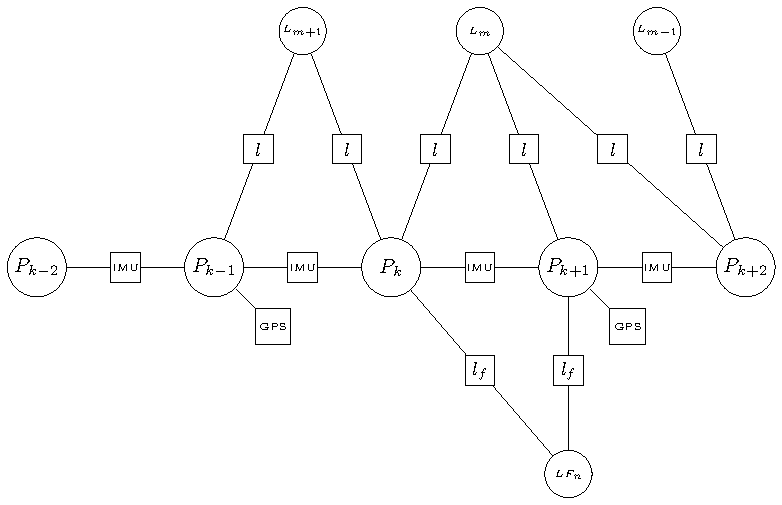
\includegraphics[scale=0.4]{./../factor_graph/factor_graph.pdf}};
\node at (10,8) {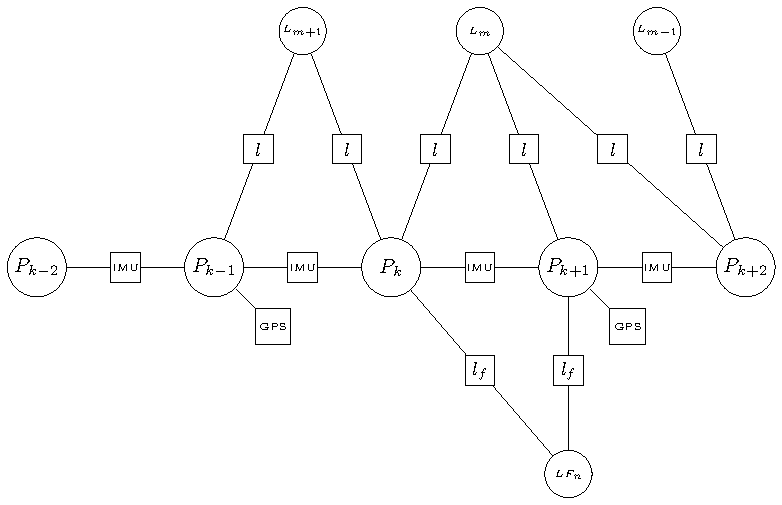
\includegraphics[scale=0.2]{./../factor_graph/factor_graph.pdf}};


%% TODO add it below \end
%\caption{Do not forget!
%Make it explicit enough that readers
%can figure out what you are doing.}

\draw [ultra thick, rounded corners, purple] (5.5,8.5) ellipse (0.5 and 0.2);
\node (v1) at (5,7.1) {};
\node (v2) at (5,8.6) {};
\node (v3) at (6,8.6) {};
\node (v4) at (6,7.1) {};
\draw [ultra thick, rounded corners, purple] (v1) edge (v2);
\draw [ultra thick, rounded corners, purple] (5,7.25) arc (180:360:0.5 and 0.2);
\draw [ultra thick, rounded corners, purple] (v3) edge (v4);

\draw [->](6.75,7.701) arc (-120.0007:-60:1.5);
\draw [->](8.25,8.299) arc (59.9993:120:1.5);

\node at (5.5,7.75) {Map};

\node at (7.5,8) {Translator};

\end{tikzpicture}


    
    
    